\subsection{Settings}
The settings subsystem allows users to changed their user account information. A user can add more music accounts (SoundCloud, Spotify, etc), logout, and change the theme.

\begin{figure}[h!]
	\centering
 	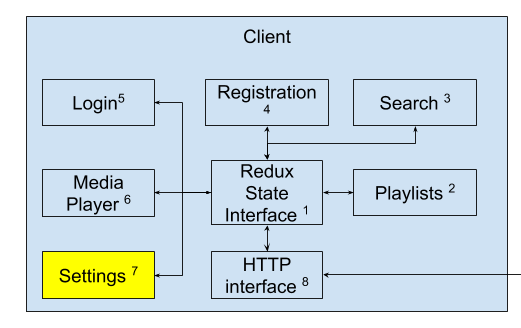
\includegraphics[width=0.60\textwidth]{images/client/client_settings.png}
 	\caption{Settings subsystem}
\end{figure}

\subsubsection{Assumptions}
One assumption made is that the user will be logged in before accessing the settings.

\subsubsection{Responsibilities}
This subsystem's primary responsibility is to allow a user to change their user information. The settings subsystem will be able to interact the with the Redux State interface to change the users theme, log them out, and add a music account to their Synthify account.

\subsubsection{Subsystem Interfaces}
\begin {table}[H]
\caption {Settings interfaces} 
\begin{center}
    \begin{tabular}{ | p{1cm} | p{6cm} | p{3cm} | p{3cm} |}
    \hline
    ID & Description & Inputs & Outputs \\ \hline
    \#01 & Redux State Interface & \pbox{3cm}{Account setting to be changed \\ user} & \pbox{3cm}{Changed setting}  \\ \hline
    \end{tabular}
\end{center}
\end{table}

\newpage
